%----------------------------------------------------------------------------------------
%	PACKETS AND CONFIGURATION
%----------------------------------------------------------------------------------------

\documentclass{report}

\usepackage{geometry}   % Edit document margins
\usepackage{hyperref}   % Table of contents hyperlinks
\usepackage{parskip}    % Paragraph indent & skip
\usepackage{graphicx}   % 'graphics' package interface
\usepackage{listings}   % Code sections formatting
\usepackage{xcolor}     % More colors
\usepackage{amsmath}    % Math

\usepackage{csquotes}   % recommended for biblatex

\usepackage[
    backend=biber,
    style=ieee,
    maxbibnames=99,
    minbibnames=3,
    maxcitenames=2,
    mincitenames=1,
    citestyle=numeric-comp,
    sorting=none,
    dashed=false
]{biblatex}             % for bibliography

% HELPER PACKAGES (REMOVE IN FINAL) %
\usepackage{todonotes}
\usepackage{blindtext}
% HELPER PACKAGES (REMOVE IN FINAL) %

% Custom Monospace + Bold command: \textttbf{"text"}
\def\textttbf#1{\renewcommand{\ttdefault}{pcr}\texttt{\textbf{#1}}\renewcommand{\ttdefault}{cmtt}}

% Custom Colors
\definecolor{AnnotationGreen}{RGB}{34, 128, 45}
\definecolor{CommentGreen}{RGB}{29, 204, 49}

% Hyperlink setup
\hypersetup{
    colorlinks,
    citecolor = blue,
    filecolor = blue,
    linkcolor = blue,
    urlcolor = blue
}

% Python code formatting
% Use it by creating an environment like \begin{lstlisting}[style=Python] ... \end{lstlisting}
% Since annotations aren't tagged as keywords I have inserted a manual delimiter for them,
% it works as follows: \@@AnnotationText@@/
\lstdefinestyle{Python}{
    language = Python,
    basicstyle = \footnotesize\ttfamily,
    commentstyle = \textcolor{CommentGreen},
    stringstyle = \textcolor{orange},
    showstringspaces = false,
    keywordstyle = \textcolor{blue},
    moredelim = [is][\textcolor{AnnotationGreen}]{\\@}{@@\/},   % Annotations
    numberstyle = \scriptsize\ttfamily\textcolor{gray},
    numbers = left,
    frame = single,
    frameround = tttt,
    framexleftmargin = 20pt,
    framexrightmargin = 20pt
}

% Setup bibliography
\addbibresource{report.bib}

%----------------------------------------------------------------------------------------
%	DOCUMENT
%----------------------------------------------------------------------------------------

\begin{document}

% TITLE
%---------------------------------------------------------------------
%   TITLE
%---------------------------------------------------------------------

% Margins for the title
\newgeometry{top=7cm, bottom=2cm} 

\begin{titlepage}
    \centering
    \vspace*{2em}
    
    % Main title
    {\Huge\bfseries Online Learning Applications \\ Advertising Project Report \par}
    
    \vspace{4em}
    
    % Professor
    {\large\scshape Prof. Nicola Gatti \par} 
    
    \vspace{3em}
    
    % Date
    {\large\slshape July 2022 \par}
    
    \vspace{3em}
    
    % Authors
    {
        \large\itshape 
        Dorian Boille
        \par
        Raul Singh
        \par
        Roberto Reggiani
        \par
        Davide Rigamonti
        \par
        Ole Martin Ødevald Ruud
        \par
    }
    
    \vfill
    
    % Polimi logo
    \begin{figure}[b]
        
\includegraphics[scale=0.6]{img/polimi.png} 
        \centering
    \end{figure}
\end{titlepage}

% Reset margins
\newgeometry{bottom=3cm} 


% ToC
{
    \hypersetup{hidelinks}
    \tableofcontents
}

% LIST OF TODOS (REMOVE IN FINAL) %
\listoftodos
% LIST OF TODOS (REMOVE IN FINAL) %

% INTRODUCTION
\chapter{Introduction}
\label{chap:introduction}


% ENVIRONMENT MODELING
\chapter{Environment modeling}

\section{Overview}
\label{chap:env_overview}

The environment is coded as a constant base upon which we build the entire project. This choice has been derived from two main reasons. \textit{The first one} is that the environment's nature doesn't change in each different step thus behaving always in the same way. \textit{The second one} is to better compare the results of different situations without introducing a bias in the inputs we feed the algorithm.

What will be changing is how much data the Learner will be given as input, this will be specified in each specific section of the document.

\section{Hypotheses}
 \label{sec:env_hypoteses}

In this section the specific assumptions related to the environment modelling are listed.

\begin{itemize}
    \item Each consumer is characterized by 2 binary features, for instance: occupation (student/worker) and gender (female/male). These features will define the 3 different user classes we want to target in our advertisement campaign.
    \item The probability for each class to be able to enter the website is fixed and known. It can be seen as the percentage over the population we are focusing with our ads.
    \item Each user class is distinguishable by an $alpha_i$ function expressing the ratio of users landing on the web-page where product $P_i$ is shown as the primary one. More clearly, given a campaign every class is characterized by a different profile of $alpha$ functions.
    \item The competitor's budget is assumed to be constant assuming a \textit{non-strategic player}.
 \end{itemize}

\section{Model Choice}
\label{sec:env_Motivation}
We chose to model the $alpha$ functions as sigmoid functions since they are constrained by a pair of horizontal asymptotes as $ x\to\pm\infty$  and this characteristic fit well the hypothesis that the maximum expected value of $alpha$ correspond to the case in which the budget allocated on that campaign is infinite. Moreover having three different parameters to attune (steepness, shift, and upper bound) gives us the possibility to better differentiate each user class.
\todo{add our motivating application and reason on why we choose prob distribution for each variable and write it better, just trying latex also default ones}

\section{Code Analysis}
\label{sec:env_Code Analysis}

The environment is composed by different objects and functions which model the users' interactions on the web-page, how users react given different budgets and it returns the final result of a day of interactions.
 
 \begin{enumerate}
     \item Enviroment data
     
     This data class contains all the environment's values. It is obtained passing by a random generation of the parameters, which are the only ones not know by hypothesis. The known parameters are set up by the data class constructor with default values as shown in the section \textbf{Model Choice}. After constructing this class, it can be passed to the function  \textit{get day of interactions}. If it needs to be set up with different values, such as an incomplete graph, it can simply be specified when the class is constructed.
    
     \item $\alpha$ functions.
     
     Computes the expected value of clicks given a certain budget for a specific function. As other parameters it needs the steepness, the shift and maximum value that characterizes the curve. Notably, the maximum value represents the maximum expected number of clicks possible.
  
    \item Generation of a graph.
    
    This function generates by default a 5x5 fully connected graph without any auto-loops. It takes as input the number of nodes with a Boolean value which decides if it needs to be fully connected or not. In the last case it is also needed another integer representing the probability to not have two nodes connecting. It returns a square matrix representing every weight between any nodes.
   
    \item Modelling user interaction.
    
    With the aid of the function \textit{get interaction} we can compute a single interaction and return the results. Taking as input the user class, the primary product's web page, a list in which it is also included also the competitor and the environment data the function returns the action taken in that specific scenario. More precisely it provides us the number of each item bought by the user belonging to the given class.
    
    This is possible throughout the function \textit{Go to page} where models the interaction between user and web-page; in fact, given a user and his class together with the Enviroment Data, it brings the user to a primary product and, if bought, behaves as expleined in section \textbf{Introduction}.
    
    \item Overall result of a day
    
    \textit{get day of interactions} gives us the interactions of a whole day and generates new updated parameters given a specific budget for each product as input. It also needs the \textit{Environment Data} and the total number of visitors of the e-commerce for that day.
    
\end{enumerate}


% OPTIMIZATION ALGORITHM
\chapter{Optimization algorithm}
\label{chap:opt_alg}

\section{Problem Formulation}
\label{sec:Opt_Problem Formulation}
Our problem, since the bidding part is out of the focus of the project, is reduced to finding the optimal budget per campaign in order to maximize the profit.
The profit is defined as the difference between the (expected margin) and the spent in advertising and it is given by the number of each product bought and (his price); since in the project's assumption the price is equal to the margin.
The number of clicks is represented by $\alpha_i$ which are influenced by how much of the budget we invest on that particular subcampaign.
Basically, it is a maximisation subject to the obvious constraint: the sum of the daily budget can't be greater then the overall budget.

\todo{clarify why price and not expected return of product,Moreover we decided to not put any lower and upper bound on subcampaign to better explore all possibilities?}

The optimization problem can be expressed as follows:
\begin{displaymath}
F=\max_{\substack{x_i\in B}} \sum_{i=0}^n \alpha_i(x_i)p_i-x_i \ s.t. \sum_{i=0}^n x_i\leq B  
\end{displaymath}
\todo{how to nicely space formulas?}

Where: 
\begin{itemize}
    \item F represents the profit defined as the difference between the expected margin and the spent in advertising.
    \item $\alpha_i$ are the value per click set equal to the expected margin from landing to the corresponding product.
    \item B is the total budget usable.
    \item $x_i$ are the money spent on the sub campaign ads for each product $P_i$.
\end{itemize}

At start we can use a dynamic-programming algorithm to optimize this function considering that all the parameters are known.
\todo{and neglecting that the budget spent is to subtract from the objective function} Furthermore, in the dynamic-programming algorithm, we can find the best way to spend the budget, for every feasible value of the budget. 
\todo{This can give us a clairvoyant result with witch we can compare other more realistic algorithm.?}

\section{Code Analysis}
\label{sec:Opt_Code Analysis}

By the aid of the function \textit{budget assignment} we solve the budget assignment problem over the value matrix representing our optimization problem. The matrix is assumed to be divided into N rows and M columns. In the rows we have the sub campaigns, in the columns we have the values of the daily budget described by fractions from 0 to B, where B is the max budget. The function considers that the sum of the returned allocations can not exceed the previous column. The value in each cell is the reward of assigning budget j to campaign i and return a vector where row i has the index of selected column j of C.

\section{Solving the Budget Assignment Algorithm}
\label{sec:budget_assignment_algorithm}

As a part of the optimization problem we utilize a dynamic programming algorithm to solve a discretized budget assignment problem. Assigning the budget in the most profitable way is similar to solving the multidimensional knapsack problem.

By first creating a matrix over the value of assigning a certain budget to a given sub-campaign. The rows of the matrix correspond to the different sub-campaigns and the columns corresponding to the different budget levels. For the algorithm to work, it is important that the columns are separated by a constant step size. As a simplification we have in our case then determined that column $j$ signifies a budget of $j * (B / M)$, where $B$ is the total budget and $M$ is the amount of columns. Put simply, the columns represent a budget fraction of the total budget.

Given this matrix, the algorithm will then find the best allocation of the budget to maximize the total value. By iterating over the rows of the matrix, and in essence taking more and more sub-campaigns into consideration, two new tables are created which store both the highest value so far and the needed allocation to achieve that value. E.g. when calculating the value for budget fraction $\frac{1}{2}$ when only the first sub-campaign is considered, the full amount of the current fraction would always be assigned to current, and only, campaign. However when the second campaign is introduced, all possible combinations of assignments between the two are considered. In that case there might be that allocating $0$ to the first and $\frac{1}{2}$ to the second gives the highest value. Then the value of this allocation is stored in the dynamic table at the second row and column of the budget fraction $\frac{1}{2}$. Lastly the second table is populated with the index of the allocation made, so in this case the index of the chosen budget fraction.

After constructing the two dynamic tables above, the last rows then consist of the situation in which all sub-campaigns are considered, hence by choosing the biggest value in this row, the best budget assignment for the entire problem is found. Using the table with the allocation indices the amount of the budget for the given campaign is stored, and the remaining budget is updated. I.e. if allocated half of the budget for the last campaign, we want to best distribute the remaining half of the budget to the other sub-campaigns.

\todo{Should we include the actual code too as a listing here?}
\todo{Should there be a visual explanation aswell (it's hard to explain in text tbh)?}


% OPTIMIZATION WITH UNCERTAIN ALPHA FUNCTIONS
\chapter{Optimization with uncertain \texorpdfstring{$\alpha$}{alpha} functions}
\label{chap:unc_alpha}


% OPTIMIZATION WITH UNCERTAIN NUMBER OF SOLD ITEMS
\chapter{Optimization with uncertain number of sold items}
\label{chap:unc_items}


% OPTIMIZATION WITH UNCERTAIN GRAPH WEIGHTS
\chapter{Optimization with uncertain graph weights}
\label{chap:unc_weights}

\section{Problem}
\label{sec:unc_w_problem}

In this scenario the only uncertain parameters are the graph weights.

Alongside the other operations, the learner will run a \textbf{graph estimation} algorithm to build an accurate representation of the graph at each time step.
Meanwhile, since the $\alpha$-functions are known, there is no need to estimate them and they can be applied directly in the optimization problem.

\section{Implementation}
\label{sec:unc_w_impl}

\subsection{Initial solution}

In the first interpretation of this assignment we set out to exploit graph influencing techniques in order to tackle this problem, however, in the long run the results were suboptimal and we decided to opt for a different approach.

Nonetheless, the graph influence related functions still exist in the codebase for posterity reasons, those are: \texttt{get\_influence\_per\_product}, \texttt{make\_influence\_graph} and \texttt{get\_influence\_of\_seed}.
The rationale for our graph influencing approach was based on determining how much each product was valuable to invest budget in by following activation patterns on the estimation of our graph, which contained our approximate weights.

In the end we opted for a more experimental approach that better exploited all of the information at our disposal in this particular step: by simulating the hypotethic behavior of a fixed set of people walking the graph, following our estimated weights and observing which products resulted in more return; we were able to produce meaningful budget assigments and tune the estimated graph weights over time following the behavior observed on real interactions.

\subsection{Prediction}

Since there is no need to estimate the $\alpha$-functions, the best allocation is calculated using the \texttt{find\_optimal\_superarm} function used to obtain the best estimation when the $\alpha$-functions are known.
The only difference is that a custom graph needs to be specified since we don't have access to the real graph weights.

\subsection{Graph estimation}

The learner contains a graph representation that is updated at each time step; the graph representation is not updated directly but through a function called \texttt{graph\_estimate}, which collects samples from various beta distributions for each graph weight, deleting \textit{self-loops} and non-existent edges.

The parameters of the beta distributions ($\alpha$ and $\beta$) are defined for each edge of the graph and represent the effective quantities that are updated whenever the function \texttt{learn} is called on the learner.

Whenever we want to make the graphless learner learn by calling its dedicated function, the learner analyzes all of the interactions given as a parameter and looks at the path that the users traversed by comparing it with the current graph representation.
If a certain edge is taken or not by a given user, the $\alpha$ and $\beta$ parameters are updated accordingly.
When \texttt{predict} is called again, the graph representation is then generated from scratch by drawing samples from the beta distributions with the updated parameters.

\subsection{Relevant code}

Implementation of the \texttt{predict} function:

\begin{lstlisting}[style=Python]
def predict(
	self, data: MaskedEnvironmentData
) -> Tuple[np.ndarray, Optional[List[List[Feature]]]]:
	budget_steps = np.linspace(0, data.total_budget, self.n_budget_steps)

	# Sample current estimation of graph
	graph = self.graph_estimation()

	best_allocation = find_optimal_superarm(data, budget_steps, custom_graph=graph)

	return budget_steps[best_allocation], None\end{lstlisting}

Implementation of the \texttt{learn} function:

\begin{lstlisting}[style=Python]
def learn(
	self, interactions: List[Interaction], reward: float, prediction: np.ndarray
):
	for interaction in interactions:
		remaining_edges = [
			(product, next_)
			for product, nexts in enumerate(self.next_products)
			for next_ in nexts
			# Only add edge to remaining if we visited the page, otherwise
			# we got no information about those edges
			if interaction.items_bought[product] > 0
		]
		for edge in interaction.edges:
			s, t = edge
			self.alpha_param[s, t] += 1
			remaining_edges.remove(edge)

		for edge in remaining_edges:
			s, t = edge
			self.beta_param[s, t] += 1
\end{lstlisting}

\section{Results}
\label{sec:unc_w_res}

\subsection{Single run reward and regret}

\begin{center}
	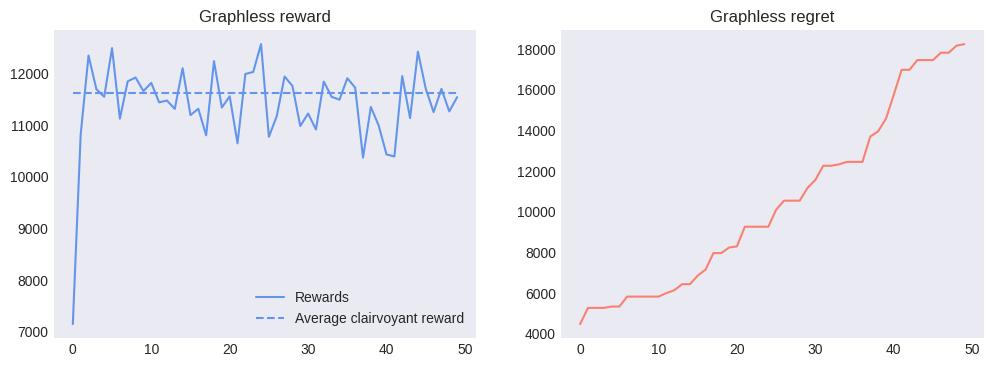
\includegraphics[scale=0.5]{img/Graphs/graphless/image1.png}
\end{center}

\subsection{Average reward and regret}

\begin{center}
	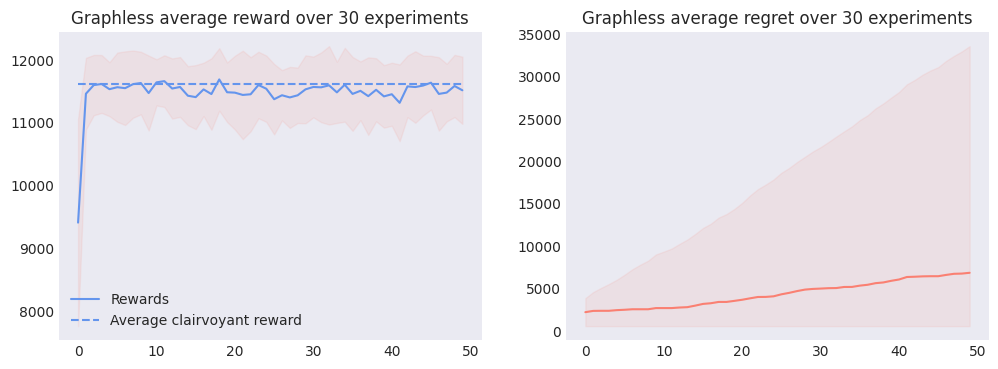
\includegraphics[scale=0.5]{img/Graphs/graphless/image2.png}
\end{center}

\subsection{Conclusions}

We can observe that the regret is exceptionally low w.r.t the previous learners, this is most likely due to the fact that the graphless learner has access to most of the important information from the environment and is able to give accurate estimations from the start.
However, some variance is always present due to the \textit{imperfect graph estimation} and \textit{environment non-determinism}.

Average results over 30 runs at time horizon $T = 50$:

\begin{table}[h]
	\center
	\begin{tabular}{|c|cc|c|}
	\hline \hline
		\cellcolor{blue!25} & Reward 	& Regret	& Deviation \\
	\cline{2-4}
		\cellcolor{blue!25} & $\mu$		& $\mu$		& $\sigma$	\\
	\hline \hline
		Graphless			& 11515.87 	& 6845.87	& 534.97 	\\
	\hline \hline
	\end{tabular}
\end{table}


% OPTIMIZATION WITH NON-STATIONARY DEMAND CURVE
\chapter{Optimization with non-stationary demand curve}
\label{chap:ns_demand}

\section{Environment behavior}

\subsection{Overview}

By using the \textbf{non-stationarity} assumption we are taking into consideration that the demand curve could be subject to changes over time and isn't necessarily fixed as we have seen in other steps.

There are 2 main types of \textit{non-stationary behaviors}:
\begin{itemize}
    \item \textbf{Abrupt changes}: where it's possible to identify different phases with different phase-wise stationary demand curves.
    \item \textbf{Smooth changes}: where the demand curve changes over time in a continuous manner.
\end{itemize}

As per specifications, we will only consider \textbf{abrupt changes} in the scope of our project.

\subsection{Abrupt changes}

\textbf{Abrupt changes} are usually experienced when an important event strikes the market \textit{(e.g. a new product that shifts the interests of the users is released or an historical event shapes the opionion of people)}; change isn't necessarily bad, however, it may impact negatively the prediction of learners that were created with a static environment in mind.

Neither \textbf{UCB} nor \textbf{TS} account for abrupt changes since it's almost impossible for them to try a superarm that was deemed as \textit{unoptimal} over the past iterations (while it might have become optimal after an \textit{abrupt change}), therefore we expect to see a significant \textbf{reward drop} from them after an \textit{abrupt change}.

In the early stages of the project we noticed that the \textbf{Simulation} that we created wasn't really fit to dinamically include abrupt changes in the environment, therefore great effort was spent in completely reworking the interface for the \textbf{Simulation} from the ground-up.

Besides collateral improvements in reproducibility, results collection and user-friendliness, the new \textbf{Simulation} allowed for an \textit{incremental simulation unfolding}, this meant that we were now able to simulate \textit{n} days, change the environment and simulate another \textit{n} days.

This particular feature revealed itself as fundamental for the upcoming challenges.

\section{Algorithms}


There are 2 main approaches to deal with a \textbf{non-stationary environment}
\begin{itemize}
    \item \textbf{Sliding window}: only consider the last $\tau$ samples for predictions.
    \item \textbf{Change detection}: detect when a change has happened and adapt accordingly.
\end{itemize}

It's clear that \textbf{Sliding window} approaches are more fit for \textbf{smooth changes} while \textbf{Change detection} approaches work better with \textbf{abrupt changes}, however it's important to note that both approaches can be utilized to deal with any \textit{non-stationary} scenario.

\subsection{Sliding window for TS and UCB}

\begin{itemize}
    \item \textbf{SW-GPTS} only differs in the \textbf{gaussian process} update since the older samples are progressively removed from the estimation as time goes on.
    \item \textbf{SW-GPUCB} also differs in the confidence bound formulation and the new arm choice:
        \begin{displaymath}
            a_t =
            \begin{cases}
                a_{\overline{t}} & \text{if} ~ \exists \overline{t} ~ | ~ n_{a_{\overline{t}}}(t-1, \tau) = 0 \\
                arg\max_{a \in A} \left\{ \mu_{t-1, \tau} + \delta \sigma_{t-1, \tau} \right\} & \text{otherwise}
            \end{cases}
        \end{displaymath}
\end{itemize}

\subsection{Change detection}

We used a \textbf{reward-based algorithm} as a \textit{change detection algorithm}, it works by comparing the last $k$ rewards with the newest $k$ rewards ($k=4$ by default) and if the difference between their means exceedes a certain threshold $\omega$ ($\omega=400$ by default) the learner is \textbf{reset} and is therefore able to learn a new optimal superarm from scratch.

Formally:
\begin{displaymath}
    \text{RESET learner if} ~ t \geq 2k ~ \land \sum_{i=t-2k}^{t-k} r_i -\sum_{i=t-k+1}^t r_i > \omega
\end{displaymath}

{\scriptsize N.B. there is an offset of 1 in the representation of t between theory and code}

\section{Results}

\subsection{-}
\todo{insert results}

\subsection{Theoretical guarantees}

In addition, if the \textbf{number of breakpoints} $m$ is small enough with respect to the \textbf{time horizon} $T$ to the power of $\alpha$ we have that the \textbf{regret} is of the order $O\left( \vert A \vert T^{\frac{1+\alpha}{2}} \right)$

\todo{adapt from import}


% CONTEXT GENERATION
\chapter{Context generation}
\label{chap:ctx_gen}

% CONCLUSIONS
\chapter{Conclusions}
\label{chap:conclusions}

% Print table of biblography references
\printbibliography

\end{document}
